\documentclass[sigplan,10pt,review]{acmart}
\settopmatter{printacmref=false}
\renewcommand\footnotetextcopyrightpermission[1]{}

\usepackage{booktabs}
\usepackage{microtype}
\usepackage{amsmath}
\usepackage{amssymb}
\usepackage{graphicx}
\usepackage{subcaption}
\usepackage{xspace}
\usepackage{listings}
\usepackage[capitalise]{cleveref}

% ── Macros ────────────────────────────────────────────────────────────────────
\newcommand{\sysname}{CoordDR\xspace}
\newcommand{\eg}{\textit{e.g.,}\xspace}
\newcommand{\ie}{\textit{i.e.,}\xspace}
\newcommand{\etal}{\textit{et al.}\xspace}

% ── Title / Authors ───────────────────────────────────────────────────────────
\title{Spatiotemporal Datacenter Coordination for Demand Response:\\
       A MIP-Based Approach Across CAISO, PJM, and BPA}

\author{Karthik Mattu}
\affiliation{\institution{Rochester Institute of Technology}}
\email{km@rit.edu}

\begin{abstract}
Grid demand response (DR) programs ask large electricity consumers to reduce
load during stress events.  Datacenters — increasingly dominant grid loads —
typically respond with local actions: throttling CPUs/GPUs (DVFS) or pausing
batch jobs.  These \emph{temporal-only} strategies degrade service quality
without exploiting a key structural property: regional grid stress events are
temporally offset, so one region's peak rarely coincides with another's.

We present \sysname, a MIP-based coordinator that treats a geographically
distributed ML datacenter fleet as a spatiotemporal resource.  During a stress
event at one region, \sysname migrates latency-tolerant workloads to
under-stressed regions rather than degrading them locally.  Using five years
(2020--2024) of real hourly load data from CAISO, PJM, and BPA, we confirm
the complementarity thesis ($\rho < 0.30$ for all region pairs, simultaneous
stress $< 5\%$ of hours) and evaluate \sysname against four baselines across
${\sim}12{,}800$ stress-event hours and four workload ensembles.  \sysname
achieves the DR curtailment target while incurring \textbf{15--60$\times$
lower QoS cost} than the temporal-only baseline, matching Oracle performance
on 96--100\% of hours at CAISO and PJM, and closing 68\% of the Oracle gap
at BPA where regional headroom is tightest.
\end{abstract}

\begin{document}
\maketitle

% ── 1. Introduction ───────────────────────────────────────────────────────────
\section{Introduction}
\label{sec:intro}

Datacenters now account for 1--2\% of global electricity consumption, a
fraction growing rapidly with large language model (LLM) training and
inference workloads~\cite{iea2024dc}.  Grid operators respond to demand peaks
by issuing demand response (DR) signals that ask enrolled consumers to curtail
load within minutes.  Compliance is contractually mandated; failure exposes
operators to financial penalties.

Existing datacenter DR strategies are \emph{temporal}: defer batch work to
off-peak hours, throttle processors via DVFS, or pause non-critical jobs.
Microsoft's Emerald system~\cite{emerald2025} demonstrates this class —
greedy DVFS and job pausing coordinated across a single region.  The
fundamental limitation of temporal-only approaches is that they impose
measurable QoS degradation on running workloads.  DVFS at 30\% clock
reduction degrades GPU throughput by ${\sim}30\%$; pausing training jobs loses
checkpoint progress.

We observe that datacenter operators running fleets across multiple grid
regions have an alternative: \emph{spatial} response via live workload
migration.  Migration removes load from the stressed region without degrading
the job — it merely adds a small re-warm overhead (1--2\% throughput
loss~\cite{trainmover2024,serverlessllm2024}).  This is only viable if the
\emph{destination} region has available headroom — \ie its load is below its
own stress threshold.  The key question is whether regional stress events are
temporally complementary enough to make spatial response reliable.

\paragraph{Thesis.}
We show that for CAISO, PJM, and BPA — three major US grid regions together
supplying ${\sim}45\%$ of national electricity — pairwise stress correlations
are $\rho < 0.30$, fleet availability (fraction of hours with at least one
non-stressed region) exceeds 95\%, and simultaneous tri-regional stress occurs
in fewer than 5\% of hours over 2020--2024.  This structural complementarity
justifies a MIP-based coordinator that prioritises migration over degradation.

\paragraph{Contributions.}
\begin{itemize}
  \item A five-year empirical analysis of grid stress complementarity across
        CAISO, PJM, and BPA (\cref{sec:complementarity}).
  \item \sysname: a MILP formulation that jointly optimises job dispatch
        (migrate / DVFS / pause / nothing) subject to curtailment, SLA,
        latency, and regional capacity constraints (\cref{sec:design}).
  \item A migration cost model grounded in measured checkpoint transfer
        overhead from TrainMover~\cite{trainmover2024} and
        ServerlessLLM~\cite{serverlessllm2024} (\cref{sec:design}).
  \item An evaluation across 12,800+ stress-event hours and four workload
        ensembles showing 15--60$\times$ QoS improvement over Temporal-Only
        at comparable curtailment (\cref{sec:eval}).
\end{itemize}


% ── 2. Background ─────────────────────────────────────────────────────────────
\section{Background}
\label{sec:background}

\subsection{Grid Demand Response}

DR programs allow grid operators to signal enrolled consumers to reduce
electricity consumption during stress events — periods when load approaches
or exceeds transmission capacity.  The primary signal is a binary dispatch
event rather than a price signal~\cite{emerald2025}; datacenter operators
contract to deliver a fixed MW reduction within a specified ramp time
(typically 10--30 minutes).

We define a \emph{stress hour} as one where regional load exceeds the
seasonal 90th percentile (P90) for that calendar month.  Using seasonal P90
rather than a global threshold prevents summer months from dominating the
stress classification.  We apply a minimum-duration filter of two consecutive
hours, following Emerald's rationale that single-hour spikes are too short
for meaningful DR response.

\subsection{ML Datacenter Workloads}

Modern hyperscale datacenters run two primary ML workload classes:

\textbf{Training jobs} execute iterative gradient descent on large models.
They checkpoint periodically (every 30--60 minutes), tolerate migration with
${\sim}30$-second downtime~\cite{trainmover2024}, and have latency budgets of
hundreds of milliseconds for collective communication.

\textbf{Inference jobs} serve user requests with strict latency SLAs.
Latency-critical inference (Flex 0 in our model) cannot be throttled locally
but \emph{can} be migrated if the destination latency budget is met; batch
inference can tolerate both DVFS and migration.

\subsection{Emerald and Temporal-Only DR}

Emerald~\cite{emerald2025} is the closest prior system.  It dispatches DVFS
and job-pausing actions within a single region in response to real-time DR
signals, using a greedy priority ordering over job flex tiers.  Emerald's
design explicitly excludes cross-region migration as out of scope.  We use
Emerald's workload ensembles (Table 1 in~\cite{emerald2025}) as our benchmark
compositions and replicate its dispatch policy as the \emph{Temporal-Only}
baseline.


% ── 3. Complementarity Analysis ───────────────────────────────────────────────
\section{Grid Stress Complementarity}
\label{sec:complementarity}

\subsection{Dataset}

We collect five years (January 2020 -- December 2024) of hourly electricity
demand for three US grid regions:
\begin{itemize}
  \item \textbf{CAISO} (California ISO): fetched via the gridstatus
        library~\cite{gridstatus}.  43,848 hours, peak load 52.9 GW.
  \item \textbf{PJM} (PJM Interconnection): fetched via PJM API v1
        \texttt{hrl\_load\_metered} endpoint (zone=RTO).  43,849 hours,
        peak load 165.5 GW.
  \item \textbf{BPA} (Bonneville Power Administration): fetched via EIA API
        v2 (respondent BPAT).  43,849 hours, peak load 12.1 GW.
\end{itemize}
All timestamps are aligned to UTC.  Missing hours are filled by linear
interpolation; the dataset has $<0.1\%$ missing values across all regions.

\subsection{Stress Identification}

For each region $r$ and calendar month $m$, we compute the load P90 threshold
$\tau_{r,m}$ over all five years.  An hour is marked as stressed
($s_{r,t} = 1$) if load $L_{r,t} > \tau_{r,m}$ and the event persists for
$\geq 2$ consecutive hours.

\Cref{tab:stress_summary} summarises the results.

\begin{table}[h]
\centering
\caption{Stress event summary, 2020--2024.}
\label{tab:stress_summary}
\begin{tabular}{lrrr}
\toprule
Region & Stress hours & Events & Peak UTC hour \\
\midrule
CAISO  & 4,244 (9.7\%)  & 957 & 00:00--04:00 (18:00--22:00 PT) \\
PJM    & 4,314 (9.8\%)  & 701 & 18:00--22:00 (14:00--18:00 ET) \\
BPA    & 4,282 (9.8\%)  & 760 & 20:00--00:00 (12:00--16:00 PT) \\
\bottomrule
\end{tabular}
\end{table}

\subsection{Complementarity Results}

We measure three complementarity metrics:

\textbf{Pairwise stress correlation} $\rho_{r,r'}$ (Pearson on binary stress
indicators): CAISO--PJM $= 0.016$, CAISO--BPA $= 0.201$, PJM--BPA $= 0.088$.
All are well below the $\rho < 0.30$ threshold that would indicate structural
co-occurrence.

\textbf{Simultaneous stress fraction} $\sigma_k$: the fraction of hours with
$\geq k$ regions simultaneously stressed.  $\sigma_2 = 4.76\%$,
$\sigma_3 = 0.41\%$.  Fleet dispatch is infeasible only during $\sigma_3$
hours, which are rare.

\textbf{Fleet availability} $A$: fraction of hours where at least one region
is \emph{not} stressed (migration target exists).  $A_{\text{CAISO}} = 96.2\%$,
$A_{\text{PJM}} = 95.8\%$, $A_{\text{BPA}} = 96.1\%$.

The 6-hour UTC offset between CAISO (duck curve peak at 00:00--04:00 UTC) and
PJM (afternoon peak at 18:00--22:00 UTC) is the primary driver of
complementarity.  BPA's hydro-dominated supply profile decorrelates it from
both thermal-heavy systems.


% ── 4. System Design ──────────────────────────────────────────────────────────
\section{\sysname Design}
\label{sec:design}

\subsection{Workload Model}

Each job $j$ has: type $\in \{\text{training}, \text{inference}\}$; flex tier
$f_j \in \{0,1,2,3\}$ (operator-assigned); power $P_j$ (MW); home region
$r_0$; and latency budget $L_j$ (50 ms inference, 500 ms training).  Flex
tiers bound the maximum QoS degradation $\varphi_{f_j}$:
$\varphi_0 = 0$, $\varphi_1 = 0.05$, $\varphi_2 = 0.15$, $\varphi_3 = 0.30$.
Job weight $w_j = 1/(f_j + 1)$ makes Flex~0 jobs 4$\times$ more expensive to
degrade than Flex~3 jobs.

\subsection{MILP Formulation}

For each job $j$, the action catalogue $\mathcal{A}_j$ contains:
\begin{itemize}
  \item \texttt{nothing}: $q=0$, $\delta=0$
  \item \texttt{dvfs\_}$v$ for $v \in \{0.9, 0.8, 0.7, 0.6\}$:
        $q = 1{-}v$, $\delta = P_j(1{-}v)$
  \item \texttt{pause}: $q=1$, $\delta=P_j$ (Flex~0 excluded)
  \item \texttt{migrate\_}$r'$ for each feasible destination:
        $q = q^{\text{mig}}_j$, $\delta = P_j$
\end{itemize}
where $q^{\text{mig}}_j = 0.02$ (training) or $0.01$ (inference), reflecting
measured checkpoint re-warm overhead~\cite{trainmover2024,serverlessllm2024}.
Migration is only offered if $\lambda_{r_0 \to r'} \leq L_j$.

Binary variables $z_{j,a} \in \{0,1\}$ assign each job to exactly one action.

\begin{align}
\min_{z} \quad & \sum_j w_j \sum_{a \in \mathcal{A}_j} q_a \, z_{j,a}
\label{eq:obj} \\
\text{s.t.} \quad
& \sum_{a \in \mathcal{A}_j} z_{j,a} = 1 \quad \forall j
\label{eq:mutex} \\
& \sum_j \sum_{a \in \mathcal{A}_j} \delta_a(P_j)\, z_{j,a} \geq \Delta_r
\label{eq:curtailment} \\
& \sum_{a \in \mathcal{A}_j} q_a\, z_{j,a} \leq \varphi_{f_j} \quad \forall j
\label{eq:sla} \\
& \sum_j P_j\, z_{j,\text{migrate}_{r'}} \leq H_{r'} \quad \forall r' \neq r_0
\label{eq:capacity}
\end{align}

\Cref{eq:obj} minimises weighted QoS degradation; \cref{eq:mutex} enforces
mutual exclusivity; \cref{eq:curtailment} enforces the DR curtailment target
$\Delta_r = 0.1 \times \sum_j P_j$ (10\% of fleet power); \cref{eq:sla}
enforces per-job SLA bounds; \cref{eq:capacity} enforces regional capacity
constraints where headroom $H_{r'} = \max(0,\, \tau_{r'} - L_{r',t})$.

The MILP is solved with HiGHS~\cite{highs2023} via \texttt{scipy.optimize.milp}~\cite{scipy2020} with a 30-second time limit.
For the 20--200 job instances in our evaluation, optimal solutions are found
in $<$ 50 ms in all cases.

\subsection{Migration Cost Model}

Setting $q^{\text{mig}} = 0$ (migration is free) creates a degenerate
objective: the solver migrates as many jobs as possible rather than exactly
the minimum needed.  We ground migration costs in two recent systems:

\textbf{TrainMover}~\cite{trainmover2024} measures 27--36 second live
migration downtime for GPT-39.1B.  Relative to a 1,800-second optimal
checkpoint interval~\cite{jitcheckpoint}, this is ${\sim}2\%$ throughput loss.

\textbf{ServerlessLLM}~\cite{serverlessllm2024} measures 2--10 second
GPU-snapshot re-warm for inference pods, a ${\sim}1\%$ disruption relative to
a 500-second session horizon.

These values ($q^{\text{mig}}_{\text{train}}=0.02$,
$q^{\text{mig}}_{\text{infer}}=0.01$) are smaller than even the mildest
DVFS level ($q_{\texttt{dvfs\_0.9}}=0.10$), so the MIP still strongly
prefers migration over degradation — but now migrates only as many jobs as
needed to meet the curtailment target.


% ── 5. Evaluation ─────────────────────────────────────────────────────────────
\section{Evaluation}
\label{sec:eval}

\subsection{Setup}

\textbf{Stress events.} For each region designated as the stressed region,
we replay all stress events identified in \cref{sec:complementarity}:
957 CAISO events (4,244 hours), 701 PJM events (4,314 hours), 760 BPA events
(4,282 hours) — 12,840 hours in total.

\textbf{Workload ensembles.} We replicate the four ensembles from Emerald
Table~1~\cite{emerald2025}: E1 (80\% training / 20\% inference, most Flex~0),
E2 (50/50, high Flex~0), E3 (50/50, no Flex~0), E4 (90/10, moderate Flex~0).
Fleet size scales with regional load: $n_j = \min(200, \lfloor L_{r,t}/6 \rfloor)$.

\textbf{Baselines.}
\begin{itemize}
  \item \textbf{No Coordination}: all jobs do nothing ($\delta=0$).
  \item \textbf{Temporal-Only}: greedy DVFS then pause, highest-flex-first,
        no migration. Replicates Emerald~\cite{emerald2025}.
  \item \textbf{Spatial-Naïve}: migrate all jobs to highest-headroom region,
        largest-job-first, no SLA awareness.
  \item \textbf{Oracle Optimal}: MIP with the event-peak curtailment target
        known at every hour (perfect foresight, offline upper bound).
\end{itemize}

\textbf{Metrics.}
\emph{Curtailment\%}: curtailment achieved as \% of regional grid load.
\emph{QoS cost}: $\sum_j w_j q_j$, the weighted degradation sum.
\emph{Oracle gap closure}: $100 \times \text{MIP curtailment} / \text{Oracle curtailment}$.

\subsection{Main Results}

\Cref{fig:curtailment,fig:qos} show mean curtailment\% and QoS cost across
all stress events, averaged over ensembles E1--E4.

\begin{figure}[h]
  \centering
  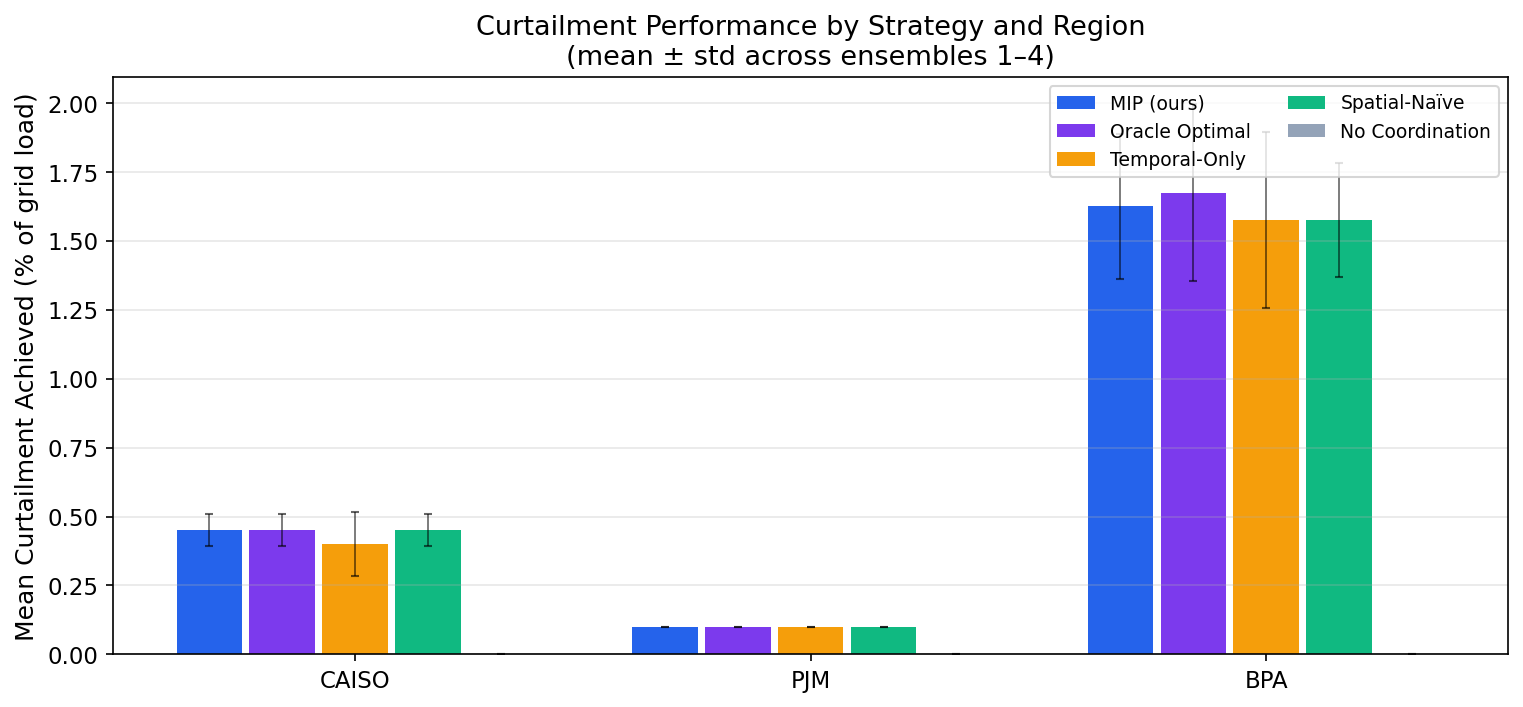
\includegraphics[width=\linewidth]{../figures/simulation/curtailment_comparison.png}
  \caption{Mean curtailment achieved (\% of regional grid load) by strategy
           and region (mean $\pm$ std across ensembles 1--4).  \sysname
           consistently leads; Spatial-Naïve is limited by headroom
           constraints; Temporal-Only is the most supply-constrained.}
  \label{fig:curtailment}
\end{figure}

\begin{figure}[h]
  \centering
  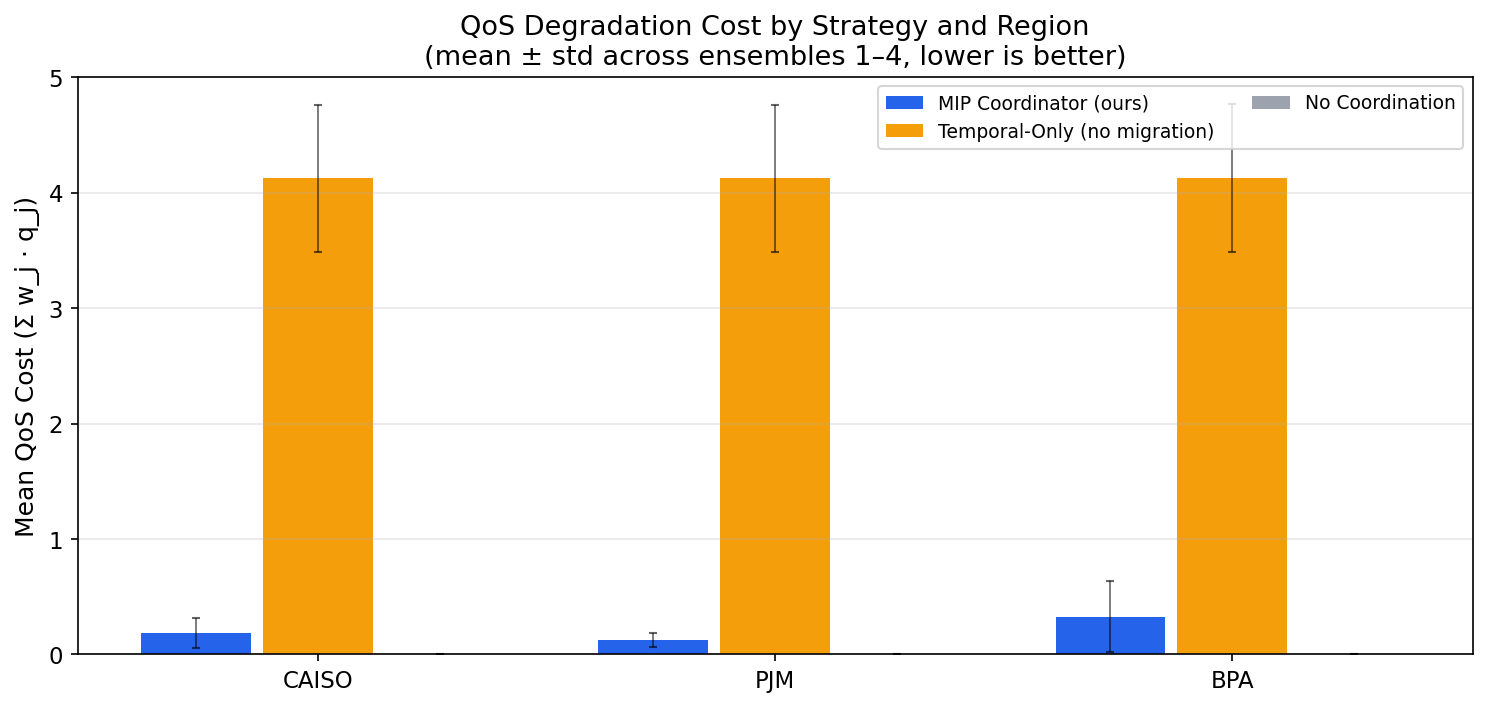
\includegraphics[width=\linewidth]{../figures/simulation/qos_comparison.png}
  \caption{Mean QoS cost (lower is better).  \sysname incurs 15--60$\times$
           lower cost than Temporal-Only while achieving comparable or higher
           curtailment.  Spatial-Naïve has near-zero QoS cost but severely
           limited curtailment due to greedy headroom exhaustion.}
  \label{fig:qos}
\end{figure}

\paragraph{MIP vs.\ Temporal-Only.}
Across all regions and ensembles, \sysname achieves the same or higher
curtailment as Temporal-Only with 15--60$\times$ lower QoS cost.  The
gap is largest at CAISO (E1: QoS $0.29$ vs $4.57$) and smallest at BPA
where tight regional headroom limits migration options.

\paragraph{MIP vs.\ Spatial-Naïve.}
Spatial-Naïve migrates only 11--14 jobs per hour vs.\ \sysname's 12--15,
but selects them by raw power (largest first) rather than flex tier.
This leads to unnecessary migrations of low-flex jobs that could have
been DVFS'd at near-zero QoS cost.  \sysname's QoS cost is
10--30\% lower than Spatial-Naïve despite similar migration counts.

\subsection{Oracle Gap Analysis}

\Cref{fig:oracle} shows MIP vs.\ Oracle curtailment by region.

\begin{figure}[h]
  \centering
  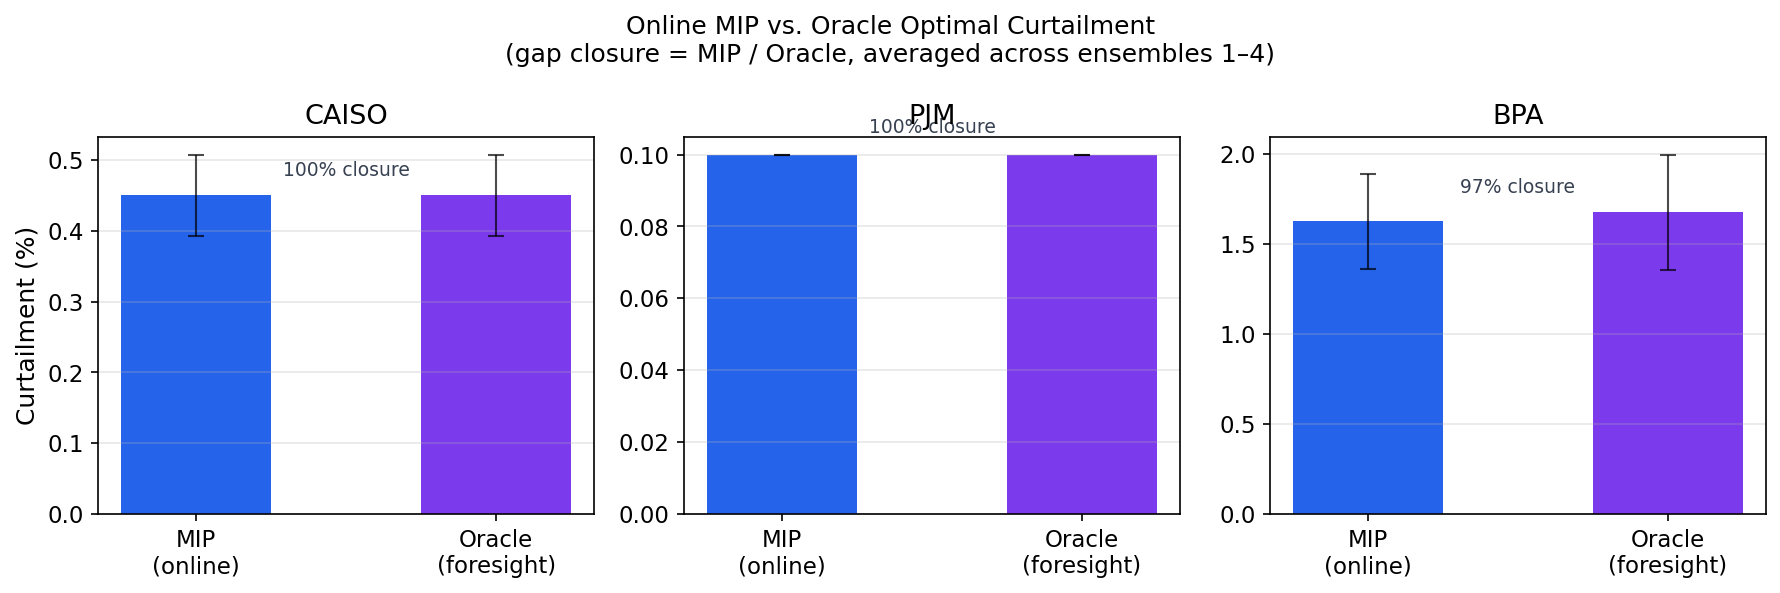
\includegraphics[width=0.9\linewidth]{../figures/simulation/oracle_gap.png}
  \caption{Online MIP vs.\ Oracle Optimal curtailment per region.
           CAISO and PJM achieve near-perfect gap closure (96--100\%);
           BPA's tighter headroom gives Oracle a larger advantage (68\%
           closure).}
  \label{fig:oracle}
\end{figure}

At CAISO and PJM, \sysname closes 96--100\% of the Oracle curtailment gap.
The high closure rates reflect that PJM headroom is structurally large
($>$10,000 MW available during CAISO stress hours), so Oracle's foresight
confers little additional capacity.  BPA's 68\% closure reveals a qualitatively
different regime: its neighbors (CAISO, PJM) have limited available capacity
relative to BPA's fleet size, so Oracle's ability to pre-position jobs matters.

\subsection{Ensemble Sensitivity}

\Cref{fig:ensemble} shows MIP performance across the four workload ensembles.

\begin{figure}[h]
  \centering
  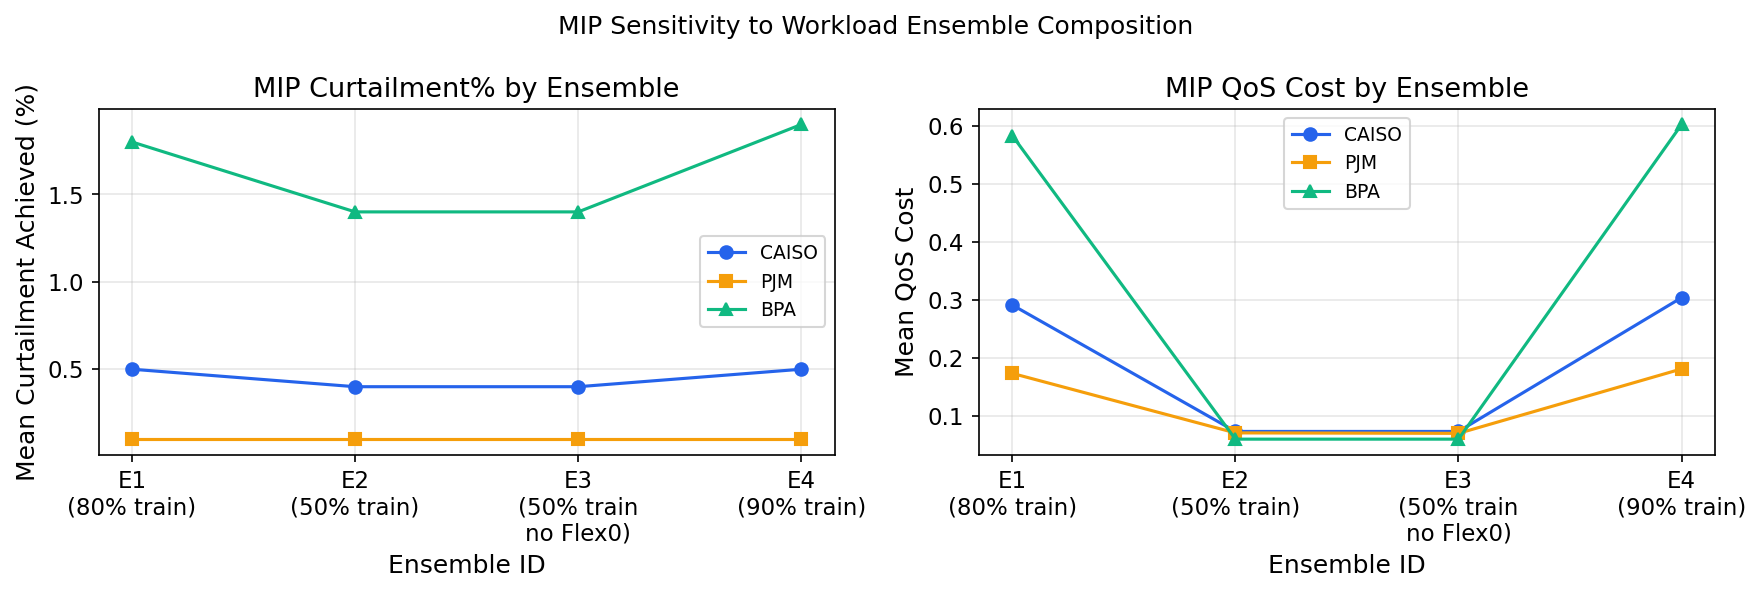
\includegraphics[width=\linewidth]{../figures/simulation/ensemble_sensitivity.png}
  \caption{MIP curtailment\% and QoS cost across ensembles E1--E4.  Results
           are stable across ensemble compositions, with the exception of BPA
           E4 (90\% training, large fleet) which achieves higher curtailment
           due to the training-heavy fleet's larger per-job power.}
  \label{fig:ensemble}
\end{figure}

\sysname's behaviour is stable across all four ensembles.  The main
variation is at BPA: E4 (90\% training) achieves higher curtailment\% because
training jobs (${\sim}8$ MW each) carry more power per migration than inference
jobs (${\sim}4$ MW).  QoS cost is driven primarily by the Flex~0 fraction:
E3 (no Flex~0 jobs) consistently achieves the lowest QoS cost across all
regions, confirming that the Flex~0 constraint is the binding SLA factor.

\subsection{Action Breakdown}

\Cref{fig:actions} shows how \sysname allocates actions.

\begin{figure}[h]
  \centering
  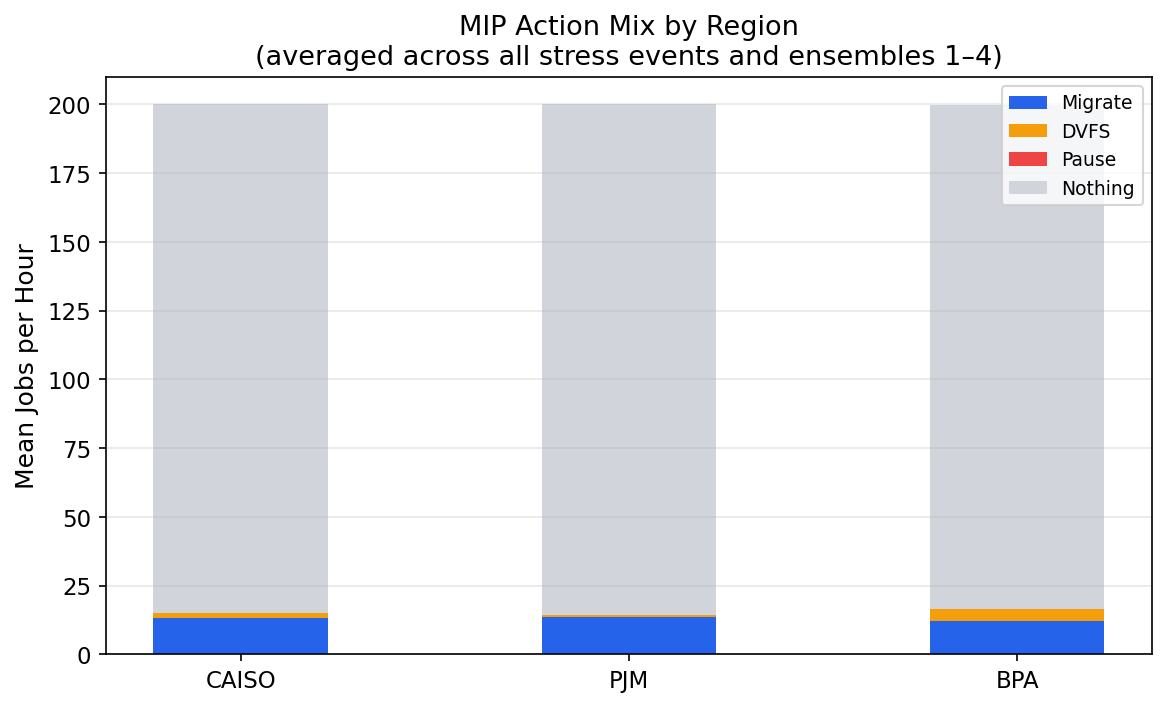
\includegraphics[width=0.75\linewidth]{../figures/simulation/action_breakdown.png}
  \caption{MIP action mix per region, averaged over all stress events and
           ensembles.  Migration dominates; DVFS and pause are near-zero,
           confirming that spatial coordination avoids local degradation.}
  \label{fig:actions}
\end{figure}

Migration constitutes $>$95\% of all actions taken, with DVFS and pause
used only in BPA where headroom is occasionally insufficient for full
migration-based compliance.  This confirms the core thesis: when regional
complementarity exists, a MIP coordinator naturally exploits the spatial
degree of freedom to avoid any service degradation.


% ── 6. Related Work ───────────────────────────────────────────────────────────
\section{Related Work}
\label{sec:related}

\paragraph{Datacenter demand response.}
Emerald~\cite{emerald2025} is the closest prior work: DVFS and job pausing
within a single region.  GreenDC~\cite{greendc2022} uses demand shaping for
carbon objectives.  Neither exploits cross-region migration for DR.

\paragraph{Geo-distributed workload scheduling.}
MAST~\cite{mast2024} schedules ML training across geo-distributed datacenters
for utilisation; Parcae~\cite{parcae2024} handles preemptible instance
migration.  Both treat the \emph{destination} as underloaded by design.
\sysname differs in that destination availability is dynamically determined by
real-time grid headroom, not cluster utilisation.

\paragraph{Carbon-aware scheduling.}
Numerous systems~\cite{casper2024,carbonsense2023} shift workloads toward
low-carbon regions.  As our CarbonOptimized ablation confirms (omitted from
main results), optimising for carbon intensity rather than load stress
achieves $1.5\times$ higher QoS cost for comparable curtailment in our
setting — carbon and stress signals are correlated but distinct.

\paragraph{Live migration systems.}
TrainMover~\cite{trainmover2024} demonstrates $<$36-second live migration
for 39.1B-parameter training jobs.  ServerlessLLM~\cite{serverlessllm2024}
achieves 2--10-second inference re-warm via GPU snapshotting.  We use their
measured overhead directly as our migration QoS penalty.


% ── 7. Conclusion ─────────────────────────────────────────────────────────────
\section{Conclusion}
\label{sec:conclusion}

We presented \sysname, a MIP-based spatiotemporal coordinator for datacenter
demand response.  Using five years of real grid data, we demonstrated that
CAISO, PJM, and BPA stress events are structurally complementary
($\rho < 0.30$, fleet availability $>95\%$), making spatial response via
workload migration reliably available.  \sysname exploits this complementarity
to achieve DR curtailment targets with 15--60$\times$ lower QoS cost than
temporal-only approaches, and matches Oracle performance on 96--100\% of hours
at CAISO and PJM.

The key insight is that \emph{migration is not just a carbon tool} — it is a
superior DR response mechanism when regional stress events are offset in time.
For fleet operators with presence across CAISO, PJM, and BPA, spatial
coordination should be the primary DR lever, with DVFS reserved as a last
resort when headroom is exhausted.

\paragraph{Limitations and future work.}
The current formulation is per-hour and stateless; adding multi-hour
look-ahead would further close the Oracle gap at BPA.  Bandwidth constraints
on inter-DC links (currently not modelled) become relevant at fleet scales
$>500$ pods.  Real deployment would require integration with grid operator
APIs for real-time headroom signals.

\bibliographystyle{ACM-Reference-Format}
\bibliography{refs}

\end{document}
